\documentclass[a4paper, 12pt]{article}
\usepackage[utf8]{inputenc}
\usepackage[spanish]{babel}
\usepackage{url, hyperref}
\usepackage[table]{xcolor}
\usepackage{adjustbox}
\usepackage{listings, xcolor}
\usepackage{graphicx, subcaption}

\definecolor{codegreen}{rgb}{0,0.6,0}
\definecolor{codegray}{rgb}{0.5,0.5,0.5}
\definecolor{codepurple}{rgb}{0.58,0,0.82}
\definecolor{backcolour}{rgb}{0.95,0.95,0.92}

\lstdefinestyle{mystyle}{
    backgroundcolor=\color{backcolour},   
    commentstyle=\color{codegreen},
    keywordstyle=\color{magenta},
    numberstyle=\tiny\color{codegray},
    stringstyle=\color{codepurple},
    basicstyle=\ttfamily\footnotesize,
    breakatwhitespace=false,         
    breaklines=true,                 
    captionpos=b,                    
    keepspaces=true,                 
    numbers=left,                    
    numbersep=5pt,                  
    showspaces=false,                
    showstringspaces=false,
    showtabs=false,                  
    tabsize=2
}
\lstset{style=mystyle, language=Python}
\setlength{\parindent}{0pt}
\setlength{\parskip}{12pt}

\title{\vspace{-3cm}Tarea 6: Ejercicio GA con función Rastrigin}
\author{
    Universidad Autónoma de San Luis Potosí\\ 
    Facultad de Ingeniería - Ing. en Sistemas Inteligentes\\ 
    \textbf{Materia:} Cómputo Bioinspirado \\
    \textbf{Prof:} Dr. Cesar Augusto Puente Montejano  \\
    \textbf{Autor:} Angel de Jesús Maldonado Juárez
}
\date{\textbf{Fecha de entrega:} jueves 20 de octubre de 2022}


\begin{document}
\maketitle

\begin{center}
    \rule{\textwidth}{0.5pt}
    \begin{abstract}
        \noindent En la naturaleza existen muchos procesos que pueden ser utilizados como una fuente de soluciones comprobadas, la evolución de los seres vivos y la selección natural son procesos comprobados para solucionar el problema de la \emph{adaptación}. Los \emph{algoritmos genéticos} (GA), utilizan estos procesos naturales para simular la evolución y selección de individuos artificiales cuyo propósito es explorar su espacio para encontrar la solución más óptima a un problema. En este reporte se muestra la implementación y configuración del algoritmo genético en Python, utilizando la librería \emph{geneticalgoritm}, para encontrar la minimización de la función \emph{Rastrigin} con 10 variables.
    \end{abstract}
    \rule{\textwidth}{0.5pt}
\end{center}

\section{Algoritmos Genéticos}
La idea principal de los algoritmos genéticos es generar \emph{individuos artificiales} (soluciones) que sean sometidos a los mismos procesos naturales de \emph{selección}, \emph{mutación}, y \emph{adaptación} en un \emph{entorno} o \emph{espacio}, también es artificial, que representa un problema que se desee resolver. Este espacio en el que las entidades (soluciones) \emph{existen}, engloba las distintas posibilidades que los individuos pueden explorar, y al momento de probar la supervivencia de la población en el espacio del problema existirá una \emph{función de evaluación} que indica, numéricamente, qué tan óptimo es la genética de cada individuo de la población para encontrar una solución (\emph{fitness}). Posteriormente, se hará una selección de individuos con base en el valor \emph{fitness} que estos recibieron, aquellos que fueron seleccionados se reproducirán entre sí utilizando algún \emph{operador genético} para generar nuevos candidatos para encontrar la solución al problema, los cuales además de tener una combinación de las características de los individuos seleccionados, también tienen características únicas gracias a la \emph{mutación}.

\section{Python + librería \emph{geneticalgorithm}}
El framework que se utiliza es \emph{Python} junto con la librería \lstinline{geneticalgorithm}, la cual utiliza la selección \textbf{estándar} y \textbf{elitista} para la implementación del GA. También cuenta con los tipos de cruzamiento \textbf{1 punto}, \textbf{2 puntos}, y \textbf{uniforme}. La función principal de la librería \lstinline{ga} puede resolver problemas \emph{continuos}, \emph{combinatorios}, y de \emph{optimización} con variables continuas, discretas, o combinadas.

Una simple modificación se realizó en la librería es en la función \lstinline{run()} de la clase \lstinline{geneticalgorithm}, donde se agregan las siguientes líneas de código para contar y mostrar el tiempo que tarda el algoritmo en calcular los resultados:

\begin{lstlisting}
timeStart = time.perf_counter()

# Algoritmo principal ...

timeEnd = time.perf_counter()
timeTotal = timeEnd - timeStart
sys.stdout.write('\n\n Total time spent: %.4f seconds' % (timeTotal))
\end{lstlisting}

\section{Función Rastrigin utilizando GA}
La función \emph{Rastrigin} es una función no convexa, que se utiliza como problema de prueba de rendimiento para algoritmos de optimización. Esta función está definida por:

\begin{equation}
    f(x)=A_n+\sum_{i=1}^n[x_i^2-Acos(2\pi x_i)]
\end{equation}

Donde $A=10$ y $x_i\in [-5.12,5.12]$.

\subsection{Implementación y configuración}
En el proyecto de \emph{Python} esta función se define con el siguiente código en el archivo \lstinline{rastrigin.py}:

\lstinputlisting{src/Python/rastrigin.py}

La función \lstinline{rastriginfcn()} es la que representa el espacio del problema que los individuos deberán de explorar.

Antes de establecer los parámetros del algoritmo, se requieren importar las librerías \lstinline{geneticalgorithm} y \lstinline{matplotlib}, la primera para utilizar el GA, y la segunda para que se puedan mostrar gráficamente la evolución del algoritmo:

\begin{lstlisting}
from geneticalgorithm import geneticalgorithm as ga
import matplotlib.pyplot as plt
\end{lstlisting}

La función \lstinline{ga()} de la librería \lstinline{geneticalgorithm} requiere de un objeto definido con las propiedades que determinan la configuración del algoritmo, el objeto \lstinline{params} guarda tal configuración, la cual es modificada varias veces para encontrar la solución (población) más óptima, la siguiente configuración tiene valores en los parámetros que \lstinline{ga()} toma por defecto:

\begin{lstlisting}
params = {\
    'max_num_iteration': None,\
    'population_size': 100,\
    'mutation_probability': 0.1,\
    'elit_ratio': 0.01,\
    'crossover_probability': 0.5,\
    'parents_portion': 0.3,\
    'crossover_type': 'uniform',\
    'max_iteration_without_improv': None\
}
\end{lstlisting}

Posteriormente, se definen la variable \lstinline{nvar}, que indica el número de variables para la función Rastrigin, y \lstinline{varbound}, que establece los límites para cada individuo de la población:

\begin{lstlisting}
nvar = 10
varbound = np.array([[-2, 2]]*nvar)
\end{lstlisting}

Finalmente, se crea el modelo para el algoritmo con la función \lstinline{ga()}, y se ejecuta con la función \lstinline{run()}:

\begin{lstlisting}
model = ga( function=rstr.rastriginfcn,\
        dimension=nvar,\
        variable_type='real',\
        variable_boundaries=varbound )

model.run()
\end{lstlisting}

\subsection{Resultados}
La siguiente tabla muestra los valores para las distintas configuraciones y resultados del algoritmo GA resolviendo la función Rastrigin ($R(x)$) con la librería \emph{geneticalgorithm} de Python:

\begin{itemize}
    \item \emph{pop\_size}: tamaño de la población.
    \item \emph{pop\_range}: rango de valores que pueden tomar los individuos de la población.
    \item \emph{mut\_prob}: probabilidad de mutación al hacer el cruzamiento.
    \item \emph{elit\_rat}: indica el porcentaje de mejores individuos que se van a utilizar.
    \item \emph{par\_port}: porción que los nuevos individuos (hijos) toman de los padres.
    \item \emph{crossover}: tipo de cruzamiento.
    \item Tiempo: tiempo que el algoritmo tarda en finalizar.
    \item Población: mejores $nvar$ individuos de la población.
    \item $R(x)$: valor que la función Rastrigin arroja con los mejores individuos de la población.
\end{itemize}

\begin{table}[!ht]
    \begin{adjustbox}{width=\textwidth}
        \begin{tabular}{|c|c|c|c|c|c|c|c|c|}
            \rowcolor{yellow}
            \hline
            $pop\_size$ & $pop\_range$    & $mut\_prob$ & $elit\_rat$ & $par\_port$ & $crossover$ & Tiempo       & $R(x)$     \\
            \hline
            $100$       & $[-2, 2]$       & $0.1$       & $0.01$      & $0.3$       & uniform     & $40.6925sec$ & $-8.9670$  \\
            \hline
            $150$       & $[-1, 1]$       & $0.1$       & $0.01$      & $0.3$       & two\_point  & $18.7244sec$ & $-10.5393$ \\
            \hline
            $150$       & $[-1, 1]$       & $0.2$       & $0.03$      & $0.9$       & one\_point  & $43.6997sec$ & $-11.1027$ \\
            \hline
            $200$       & $[-0.99, 0.99]$ & $0.4$       & $0.03$      & $0.2$       & one\_point  & $42.6043sec$ & $-12.6306$ \\
            \hline
        \end{tabular}
    \end{adjustbox}
\end{table}

Las siguientes gráficas muestran la evolución de la población en la primera corrida del algoritmo con los parámetros por defecto y un rango de $[-2, 2]$ (\ref{subfig:corrida1}), y la evolución de la población en la corrida con mejor resultado con un rango de $[-0.99, 0.99]$(\ref{subfig:corrida2}):

\begin{figure}[!ht]
    \centering
    \begin{subfigure}[b]{0.48\textwidth}
        \centering
        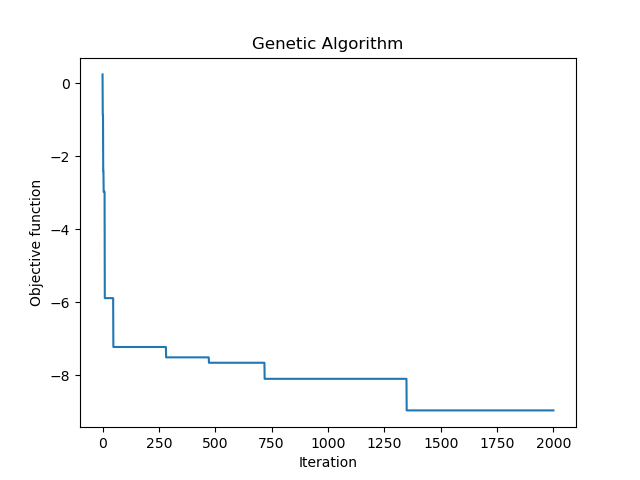
\includegraphics[width=\textwidth]{img/corrida_1.png}
        \caption{Corrida 1}
        \label{subfig:corrida1}
    \end{subfigure}
    \hfill
    \begin{subfigure}[b]{0.48\textwidth}
        \centering
        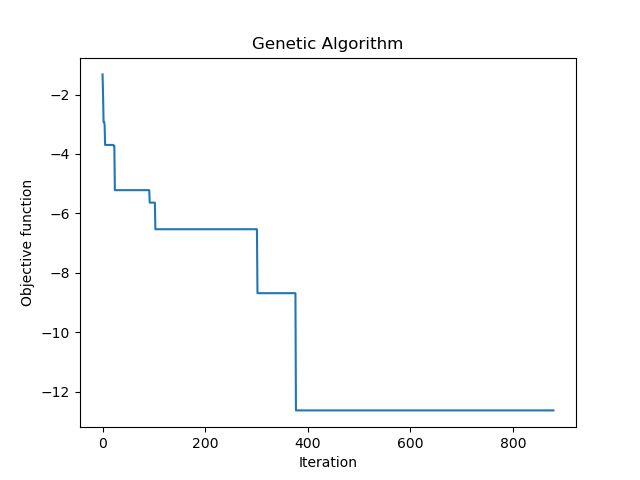
\includegraphics[width=\textwidth]{img/corrida_4.png}
        \caption{Mejor corrida}
        \label{subfig:corrida2}
    \end{subfigure}
    \caption{Primer corrida vs. mejor corrida del algoritmo GA en Python.}
\end{figure}

Los valores obtenidos (población) para las 10 variables en la primer corrida (\ref{subfig:corrida1_pob}) y la mejor corrida (\ref{subfig:corrida2_pob}) fueron los siguientes:

\begin{figure}[!ht]
    \centering
    \begin{subfigure}[b]{0.48\textwidth}
        \centering
        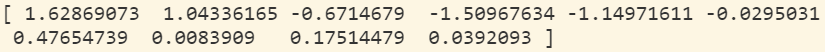
\includegraphics[width=\textwidth]{img/corrida_1pob.png}
        \caption{Mejor población corrida 1}
        \label{subfig:corrida1_pob}
    \end{subfigure}
    \hfill
    \begin{subfigure}[b]{0.48\textwidth}
        \centering
        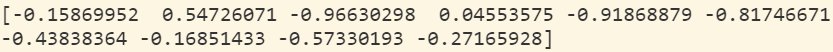
\includegraphics[width=\textwidth]{img/corrida_4pob.png}
        \caption{Mejor población obtenida}
        \label{subfig:corrida2_pob}
    \end{subfigure}
    \caption{Primer población vs. mejor población del algoritmo GA en Python.}
\end{figure}

Cabe mencionar que para la mejor corrida (\ref{subfig:corrida2} y \ref{subfig:corrida2_pob}) se modificaron también las condiciones de paro \lstinline{'max_num_iteration' : 1000} y \lstinline{'max_iteration_without_improv' : 500}, para aumentar el tiempo de evolución de la población y evitar gastar más recursos.

Se puede observar tanto en la tabla como en los gráficos que conforme aumenta el tamaño de la población, hay más probabilidad de que mejore el resultado de minimización del algoritmo GA. Sin embargo, es necesario realizar un ajuste en los parámetros del algoritmo con base en el tamaño que se le dé a la población; si el tamaño de la población aumenta también el valor de \lstinline{elit_ratio} debe ser ligeramente aumentado para que existan más élites dentro de la población y los parámetros \lstinline{mutation_probability}, \lstinline{crossover_probability}, \lstinline{parents_portion}, y \lstinline{crossover_type} deben ser modificados de tal forma que haya suficiente diversidad genética para que el algoritmo no se quede atrapado en un óptimo local.

\section{Conclusiones}
El algoritmo genético es una buena alternativa para encontrar soluciones a problemas de complejidad muy alta, o que la cantidad de posibilidades aumente de forma exponencial. Y a pesar de que se dependa en gran medida del factor aleatorio que el algoritmo tiene para la generación de nuevos individuos en la población, y que estos sean quienes encuentren una mejor solución, es mucho más rápido que cualquier otro algoritmo.

\bibliographystyle{unsrt}
\bibliography{refs}
\nocite{*}
\end{document}